\chapter{Linear Methods for Regression}{} \label{chapLinearRegression}

%citazione introduttiva
\epigraph{\textit{The Earth is not flat, but the world behaves linearly, sometimes.}}{}

This chapter, together with chapters, \ref{chapLinearClassification}, \ref{cahpNonLinear}, \ref{cahpEnsemble}, introduces the so-called “supervised learning”. Differently from unsupervised learning, these algorithms train models on data to predict the value of a given feature $y$. This section addresses regression models, i.e. models targeting a real number. \footnote{The package logproj provides methods to deal with linear regression \href{https://github.com/aletuf93/logproj/blob/master/logproj/M_learningMethod/linear_models.py}{here}.} 

\section{Supervised learning} \label{supervisedLearning}
Supervised learning (predictive algorithms) are used to predict the value of an unknown variable $y$, from a training set $X$ of observations where $y$ is given for each row of $X$. This technique is useful when it is necessary to build a prediction model of the future value of $y$. If the observations contains only the feature $y$, then time series analysis (see Section \ref{secTimeSeries}) applies. When a number of features $P$ is available for each observation, together with $y$, then an option is to build a supervised learning model.

The dataset of a learning model is composed of (see Figure \ref{fig_learningTable}):
\begin{itemize}
    \item A matrix $X_{N,P-1}$ with $N$ observations of the $P-1$ predictors;
    \item A vector $y_{N,1}$ with $N$ observations of the target variable.
\end{itemize}

% INSERT fig_learningTable
\begin{figure}[hbt!]
\centering
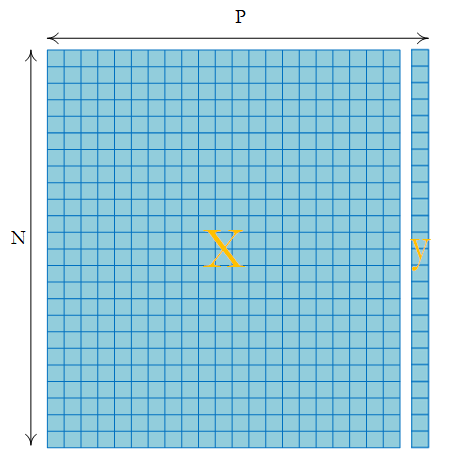
\includegraphics[width=0.7\textwidth]{SectionLetsMath/linearRegression_figures/fig_learningTable.png}
\captionsetup{type=figure}
\caption{Scheme of the input dataset of a predictive model.}
\label{fig_learningTable}
\end{figure}

Our goal is to train a model to link $X$ and $y$ efficiently. This link is the approximation of the joint probability distribution function $y=f(X)$. Predictive models are effective when they correctly estimate $f$. For validation reasons, the dataset $X$ is always split into two separate datasets:
\begin{enumerate}
    \item the training set: used to train the model;
    \item the testing set: used to test the performance of the model by measuring its error.
\end{enumerate}

The training set is needed to train the model by setting a number of parameters to maximise the fitting of the function $f$ to the data. The tuning parameters are specific for each family of models, and their value is set during the training phase. Models may have other parameters (called hyperparameters) whose values are set before the beginning of the training phase. \par
The testing set is used to compare the predictions obtained by the model with true values selected from the input dataset. If a model succeeded in this testing phase, it is ready for the implementation, i.e. to make predictions based on new data. Figure \ref{fig_trainTest} illustrates the dataflow to build a predictive model.

% INSERT fig_trainTest
\begin{figure}[hbt!]
\centering
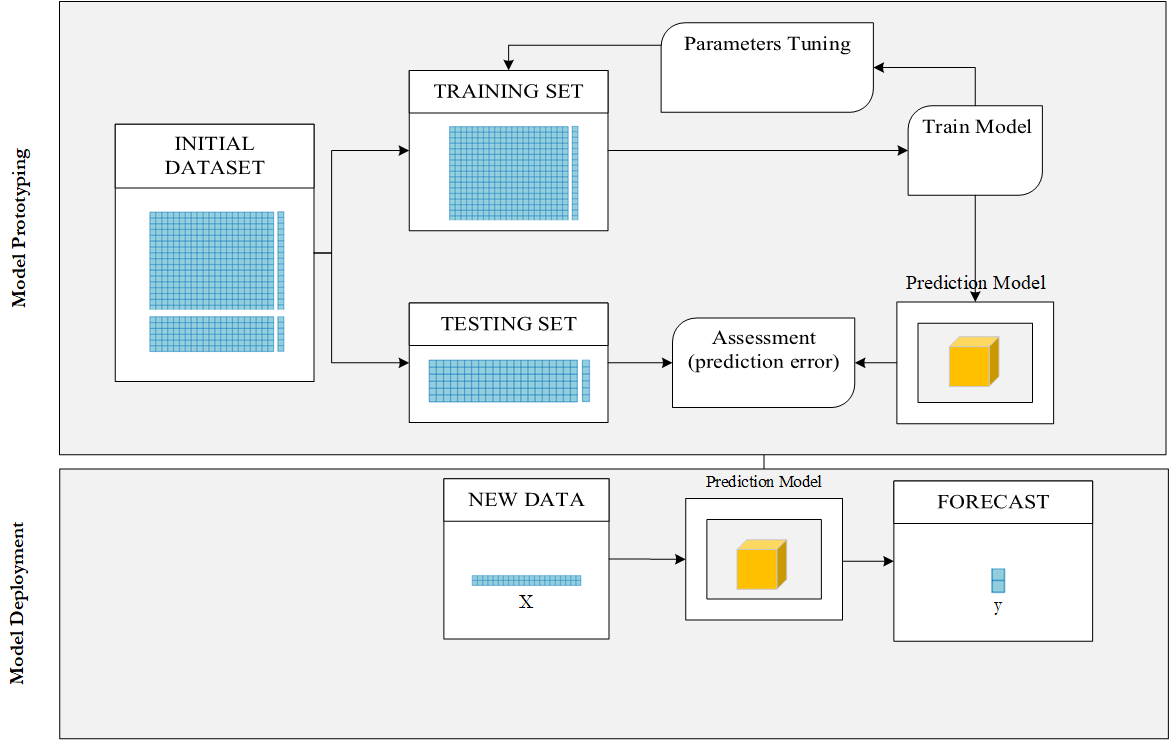
\includegraphics[width=1\textwidth]{SectionLetsMath/linearRegression_figures/fig_trainTest.png}
\captionsetup{type=figure}
\caption{Flow of the development and deployment of a prediction model.}
\label{fig_trainTest}
\end{figure}

The following chapters illustrate tens of machine learning models. It is necessary to understand how to choose the most proficient in practice. The main idea is to have an error metric and to choose the model that minimises the most this error metric. The prediction error can be calculated for the training set or the testing set. Given a training set $T$, we can define a prediction error on the training set  $\overline{err}$ and a prediction error $Err$ on the independent testing set as follows.

\begin{equation}
\overline{err}=\frac{1}{N}\sum_{i=1}^{N}L\left(y_i,f\left(x_i\right)\right)
\label{eq_trainTestError1}
\end{equation}

\begin{equation}
Err=E_{T}\left[E_{X^0,Y^0}\left[L\left(Y^0,\hat{f}(X^0)\right)|T\right]\right]
\label{eq_trainTestError2}
\end{equation}

Where $L$ is our error metric, called loss function (e.g., the mean squared error (MSE) or the absolute error). The definition of $\overline{err}$ and $Err$ shows that an error metric can always be computed for both the training and the testing set. Unfortunately, the error $\overline{err}$ measured on the training set is not a good estimate for the error $Err$ in the testing set. We want to minimise the error $Err$ on the testing set since it is the best estimate of the error that the model will have while working with new data. Stressing the minimisation of $\overline{err}$ leads to a phenomenon called \textit{overfitting}; the training error is minimised, while the training error raises.\par

A model adapts itself to best fit to the training set, but this does not imply the same good fit happens with the testing set. For this reason, it is not a good idea striving to reduce the error in the training set. In general, $\overline{err}<\ Err$ and the training error tends to zero increasing the complexity of the model (e.g., the number of features involved) but this fact does not guarantee good results of the test set.\par

Model selection involves different metrics to measure the performance of different predictive models in order to choose the best one. For this reason, the in-sample error $Err_{IN}$ is introduced to describe the error having $N$ new response values at each of the training points\footnote{This is a sampling error, i.e. a measure of how much the sample chosen to train the model represents the entire population.}.

\begin{equation}
Err_{IN}= \frac{1}{N}\sum_{i=1}^{N}E_{T}\left[E_{Y^0}\left[L\left(Y_i^0,\hat{f}(X_i)\right)|T\right]\right]
\label{eq_trainTestError3}
\end{equation}

A metrics called optimism is defined as $op=Err_{IN}-\overline{err}$. We usually consider $\omega=E_y[op]$ which can be estimated as:

\begin{equation}
\omega=\frac{2}{N}\sum_{i}^{N}{cov(\widehat{y_i},y_i)}
\label{eq_trainTestError4}
\end{equation}

The underestimation by $\overline{err}$ in the true error depends on how much $y_i$ affects its own prediction. $\omega$ is a metrics used as a basis for the evaluation of the performance of machine learning algorithms.

\subsubsection{MSE} \label{secMSE}
The most commonly used error metric to select a regression model is the mean squared error. It is calculated as:

\begin{equation}
MSE=\frac{1}{N}\sum_{i=1}^{n}\left(y_i-{\hat{y}}_i\right)^2
\label{eq_MSE}
\end{equation}

A main limitation of the MSE is that it suffers significant prediction errors on the outliers. For this reason, it is possible to introduce quantiles of errors which evaluates the error of a model within a given percentile. The mean absolute percentage error (MAPE) is used at this purpose:

\begin{equation}
MAPE=p\left(\frac{\left|y_i-{\hat{y}}_i\right|}{y_i}\right)
\label{eq_MAPE}
\end{equation}

Where $p$ is the chosen percentile. In practice, we can evaluate the percentage of estimates that differs from the true value no more than a given percentage (e.g. 10\%).

\subsubsection{AIC and BIC}

We consider $\widehat{Err_{IN}}=\overline{err}+\hat{\omega}$. Akaike information criterion (AIC) and Bayesian information criterion (BIC) are two very common metrics used to assess the performance of a model. They are defined as follows.

\begin{equation}
AIC=-\frac{2}{N}E\left[loglik\right]+\frac{2d}{N}
\label{eq_AIC}
\end{equation}

Where $loglik=\sum_{i=1}^{N}{\log(\Pr_{\hat{\theta}}{y_i})}$, $N$ is the number of samples, and $d$ defines the number of features. BIC is defined similarly.

\begin{equation}
BIC=\ -2loglik+(\log{N})d
\label{eq_BIC}
\end{equation}

Both these metrics can be used to identify the best tuning parameter of a model or to compare different models. The model with the minimum AIC or BIC value should be chosen. To choose among AIC or BIC, it is important to remember that BIC is asymptotically consistent, which is equivalent to say that BIC selects the correct model with a probability approaching 1 as $N\rightarrow\infty$. Otherwise, increasing the number of samples AIC tends to choose more complex models. In other words, BIC tends to prefer simpler models than AIC, that chooses more complex models.

\subsubsection{Cross-validation}
The metrics proposed in the previous paragraphs allows investigating the reliability of the predictions. Sometimes, when having few data, split into training, and the testing dataset may lead to very small datasets. For this reason, cross-validation (CV) or bootstrapping are used.\par

The selection of the train-test split of the data may bias these measures of the error. The CV is used to evaluate the extra-sample error $Err=E[L(Y,\hat{f}(X))]$. $K$-fold cross-validation splits the set into $K$ subsets and performs all the different permutations choosing one of them as a validation set and using the others to train the algorithms. Figure \ref{fig_crossValidation} shows an example of 5-folds CV.

% INSERT fig_crossValidation
\begin{figure}[hbt!]
\centering
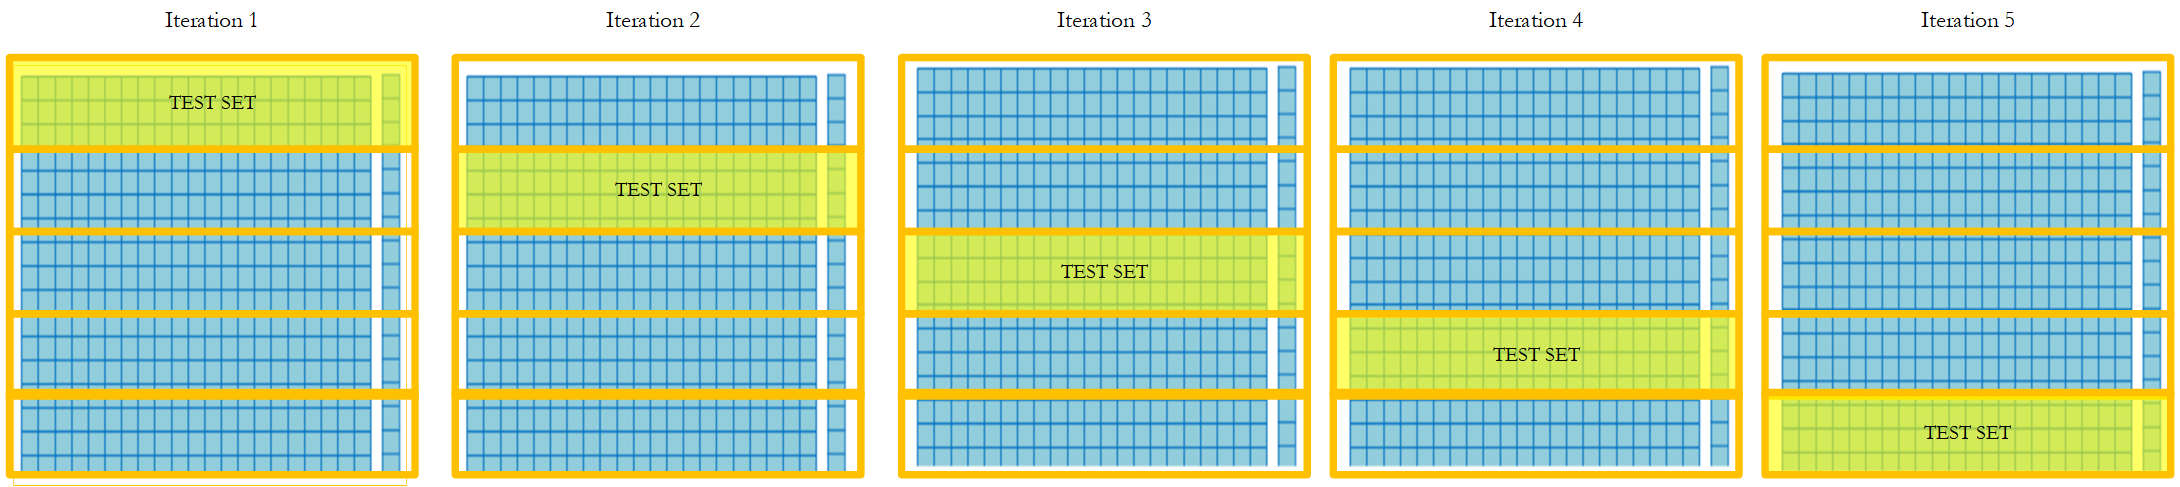
\includegraphics[width=1\textwidth]{SectionLetsMath/linearRegression_figures/fig_crossValidation.png}
\captionsetup{type=figure}
\caption{Schema of a 5-folds cross-validation.}
\label{fig_crossValidation}
\end{figure}

The CV produces an estimate of $Err$ as:

\begin{equation}
CV\left(\hat{f}\right)=\frac{1}{N}\sum_{i=1}^{N}{L(y_i,{\hat{f}}^{-k\left(i\right)}(x_i))}
\label{eq_errCV1}
\end{equation}

Where ${\hat{f}}^{-k\left(i\right)}$ is the function fitted without the $k$-th fold. A CV can also be used to choose the value of a tuning hyperparameter $\alpha$ of a model. 

\begin{equation}
CV\left(\hat{f},\alpha\right)=\frac{1}{N}\sum_{i=1}^{N}{L(y_i,{\hat{f}}^{-k\left(i\right)}(x_i,\alpha))}
\label{eq_errCV2}
\end{equation}

Besides, CV can be used together with bootstrap methods (see Section \ref{secBootstrapping}). The idea of the bootstrap is to estimate the value of the loss function. Bootstrapping samples from the empirical distribution of the data (i.e. the input dataset, since we do not know the real distribution). Bootstrap samples with replacement since a point can be added to the sampled distribution multiple times to reflect the behaviour of the empirical distribution (when sampling without replacement, we have a jackknife sampling). The error $Err$ can be estimated as:

\begin{equation}
\widehat{Err}=\frac{1}{N}\sum_{i=1}^{N}{\frac{1}{|C^{-1}|}\sum_{b\in C^{-1}}{L(y_i,{\hat{f}}^{\ast b}(x_i))}}
\label{eq_errCV3}
\end{equation}

Where $C^{-1}$ is the set of the bootstrap samples $b$ that does not contain observation $i$. 

\subsubsection{Hyperparameters tuning}

While the training phase set the values of the parameters of the model, there is no precise way to set the hyperparameters of the model. Nevertheless, hyperparameters deeply affect the prediction performance of a model. This can be done by several iterations, trying different hyperparameters values for each model. There are different strategies to tune the model\footnote{The package logproj provides grid search methods to train model, identifying the best hyperparameter \href{https://github.com/aletuf93/logproj/tree/master/logproj/M_learningMethod}{here}.}. Two strategies are:

\begin{itemize}
    \item Grid search: i.e. testing all the parameters of a given set, evaluate the performance of the model and choose the best one.
    \item Random search: random select a subsample of the grid and select the best hyperparameter among this subset.
\end{itemize}

Smart algorithms (e.g. gradient-based) exist to identify the best direction to search good values of a hyperparameter, but they are usually time-consuming and affect the total training time of the model significantly.

\section{Linear regression (OLS)} \label{secLinearRegression}

Linear regression is a predictive model assuming a linear relationship between the input $X$ and the output $y$. Let assume $X_{N,P}$ being the input matrix of $P$ features and $N$ observation, we are interested in predicting the value of the output vector $y_{N,1}$ using a linear relationship. In other terms, the linear regression works in a $P+1$-dimensional space aiming at predicting the value of $y\in \mathbb{R}$ as a linear combination of the variables $x\in \mathbb{R}^P$. In practice,we are looking for the function $f$.

\begin{equation}
f\left(X\right)=\beta_0+\sum_{j=1}^{P}{X_j\beta_J}
\label{eq_OLS1}
\end{equation}

Since $X$ is given, our problem is to define a vector $\beta$ of scalar values such that the residual sum of squares (RSS) between the values of $y$ and  $\hat{y}=f(X)$ is minimized.

\begin{equation}
\begin{split}
    RSS\left(\beta\right) & =\sum_{i=1}^{N}{\left(y_i-f\left(x_i\right)\right)^2=} \\
    & =\sum_{i=1}^{N}\left(y_i-\beta_0-\sum_{j}^{N}{x_{ij}\beta_j}\right)^2= \\
\end{split}
\label{eq_OLS2}
\end{equation}

By the definition, the sum of squares in matrix notation is the product of the transpose of a vector with the vector itself: $A^2=A^TA$; for this reason,

\begin{equation}
\begin{split}
     RSS\left(\beta\right) & = {y}^T{y}-{y}^T{X}\beta-\beta^T{X}^T{y}+\beta^T{X}^T\left({X}\beta\right)= \\
    & ={y}^T{y}-{y}^T{X}\beta-\left({X}\beta\right)^T{y}+\left({X}\beta\right)^T\left({X}\beta\right)=\\
\end{split}
\label{eq_OLS3}
\end{equation}

By the definition, $\left(AB\right)^T=B^TA^T$; then,

\begin{equation}
     RSS\left(\beta\right) = {y}^T{y}-{y}^T{X}\beta-\beta^T{X}^T{y}+\beta^T{X}^T\left({X}\beta\right)=
\label{eq_OLS4}
\end{equation}

Considering that ${y}_{1N}^T{X}_{NP}\beta_{P1}$ is a scalar number as well as $\beta_{1P}^T{X}_{PN}^T{y}_{N1}$,

\begin{equation}
     RSS\left(\beta\right) =  {y}^T{y}\ -2\beta^T{X}^T{y}+\beta^T{X}^T\left({X}\beta\right)
\label{eq_OLS5}
\end{equation}

The partial derivatives with respect to each $\beta_i (i=1,\ldots,P)$ are considered. They are all set equal to 0 to find a minimum of $RSS\left(\beta\right)$. Let define a $P\times1$ vector $e_i$ with 1 in the $i$-th position and 0 elsewhere. 

\begin{equation}
\begin{split}
     \frac{\partial RSS(\beta)}{\partial\beta_i} & =-2e_i^TX^Ty+e_i^TX^TX\beta+\beta^TX^TXe_i^T \\
    & =-2e_i^TX^Ty+{2e}_i^TX^TX\beta \\
\end{split}
\label{eq_OLS6}
\end{equation}

It is a good idea learning for a minimum since the second derivative with respect to $\beta$ is as follows.

\begin{equation}
     \frac{\partial^2RSS(\beta)}{\partial\beta}=2{X}^T{X}
\label{eq_OLS7}
\end{equation}

We can assume, by definition, that $X^TX$ is always positive if $X$ has full column rank (i.e., all its columns are linearly independent). In general, this is not true, but it is always possible to apply the PCA (see section \ref{secPCA}) to obtain an $X$ with full column rank. Given this hypothesis, $\frac{\partial RSS(\beta)}{\partial\beta}$ is set equal to 0 (for all the values of $i$) looking for a minimum.

\begin{equation}
\begin{split}
     -2e_i^TX^Ty+{2e}_i^TX^TX\beta=X^T\left(y-X\beta\right)=0 \\
     X^TX\beta=X^Ty \\
     \hat{\beta}= \left(X^TX\right)^{-1}X^Ty \\
\end{split}
\label{eq_OLS8}
\end{equation}

The equation (\ref{eq_OLS8}) defines the value of $\hat{\beta}$ which best fits the training data.

\subsection{Geometrical representation of the linear regression}
The linear nature of this model allows us to interpret the results of the previous paragraph geometrically. Equation (\ref{eq_OLS8}) proves that:

\begin{equation}
\hat{y}=X\hat{\beta}=\left(X^TX\right)^{-1}X^Ty
\label{eq_OLSgeo1}
\end{equation}

The value of $\hat{\beta}$ is found such that $X^T\left(y-X\hat{\beta}\right)=X^T\left(y-\hat{y}\right)=0$. This fact is due to the result of the derivative of the RSS $\left(\beta\right)=0$ but, by the definition of orthogonal vector, it implies the vector $y-\hat{y}$ is orthogonal to the subspace generated by the $P$ columns of $X$ (remember of the hypothesis of full column rank of $X$). In practice $\left(X^TX\right)^{-1}X^T=H$ is the function generating $\hat{y}$ as the orthogonal projection of $y$ onto the subspace of $\mathbb{R}^P$ generated by the $P$ columns of $X$ (see Figure \ref{fig_projection}).

\begin{equation}
\hat{y}=\left(X^TX\right)^{-1}X^Ty=Hy
\label{eq_OLSgeo2}
\end{equation}

% INSERT fig_projection
\begin{figure}[hbt!]
\centering
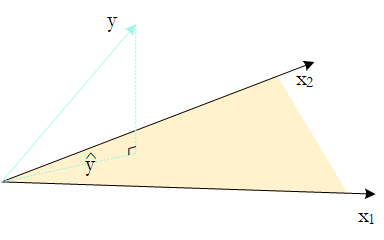
\includegraphics[width=0.7\textwidth]{SectionLetsMath/linearRegression_figures/fig_projection.png}
\captionsetup{type=figure}
\caption{Linear regression as a projection of $y$ on the space generated by $X$.}
\label{fig_projection}
\end{figure}

It is possible to take a step further considering the univariate (i.e., single variable) linear regression.

\begin{equation}
\begin{split}
Y=X\beta+\epsilon \\
\hat{\beta}=\frac{\sum_{i=1}^{N}{x_iy_i}}{\sum_{i=1}^{N}x_i^2}\\
\end{split}
\label{eq_OLSgeo3}
\end{equation}

With residuals: $r_i=y_i-x_i\hat{\beta}$. These formulae can be written as scalar products\footnote{$\langle x,y \rangle=\sum_{i}^{N}x_iw_i=x^Ty$} with vector notation. 

\begin{equation}
\begin{split}
\hat{\beta}=\frac{\langle x,y \rangle}{\langle x,x \rangle}\\
r=y-x\hat{\beta}\\
\end{split}
\label{eq_OLSgeo4}
\end{equation}

For this reason, \textit{compute a linear regression of b on a} means \textit{orthogonalize b on a} by:
\begin{enumerate}
    \item Producing the coefficient $\hat{\gamma}=\frac{\langle a,b \rangle}{\langle a,a \rangle}$;
    \item 	Producing the residuals $z=b-\ \hat{\gamma}a$.
\end{enumerate}

When dealing with multivariate linear regression, it is always possible to use this approach, applying regression by successive orthogonalization (see Algorithm \ref{algo_MultivarLinearRegression}).

\begin{algorithm}[H]
\DontPrintSemicolon
\SetAlgoLined
    
    1. 	Set $z_0=x_0=1$ \;
    2. \For{$j=1:p$}{
        	Regress $x_j$ on $z_0,z_1,\ldots,z_{j-1}$ to produce ${\hat{\gamma}}_{l,j}=\frac{\langle z_l,x_j \rangle}{\langle z_l,z_l \rangle}$ with $l=0,\ldots,j-1$ and $z_l=x_j-\sum_{k=0}^{j-1} \hat{\gamma}_{l,j}z_k$\;
    3. 	Regress $y$ on the residual $z_p$ to get  $\widehat{\beta_p}$.\;
    }
    
\caption{Multivariate linear regression}
\label{algo_MultivarLinearRegression}        
\end{algorithm}

It is clear that we are writing $x_j$ as a linear combination of $z_k$ (with $k<j$) where each $z_k$ is the additive contribution of the $j$-th parameter. Theoretically, $z_k$ are orthogonal. In case a $x_j$ is highly correlated with any of the $z_k$ (with $k<j$) the additive contribution of the residual vector $z_k$ will be close to zero (i.e. the information given by $j$-th parameter is already described by the previous $z_k$ with $k<j$).\par

There is still an open question: to identify the confidence interval of the linear coefficients $\beta_j$. To answer this question, the observations $y_i$ are assumed to be uncorrelated with constant variance $\sigma^2$. In addition, the deviation of $y$ around its mean is assumed being additive and Gaussian (i.e. additive white gaussian noise). These hypotheses allow applying some statistical test to check which of the input parameters $p$ is significant for the prediction model.\par

The variance-covariance matrix\footnote{The variance-covariance matrix is the generalization of the concept of covariance applied to a space with n variables.} is obtained as:

\begin{equation}
Var\left(\hat{\beta}\right)=\left(X^TX\right)^{-1}\sigma^2
\label{eq_OLSgeo5}
\end{equation}

The value of the variance $\sigma^2$ can be estimated by an unbiased estimator (see section \ref{secEstimators}) as follows.

\begin{equation}
{\hat{\sigma}}^2=\frac{1}{N-p-1}\sum_{i=1}^{N}\left(y_i-\widehat{y_i}\right)^2
\label{eq_OLSgeo6}
\end{equation}

Given the these hypotheses, $\beta$ is distributed as a multivariate normal distribution.

\begin{equation}
\hat{\beta}~N(\beta,\left(X^TX\right)^{-1}\sigma^2)
\label{eq_OLSgeo7}
\end{equation}

The variance can be described as a $\chi^2$ distribution with $N-p-1$ degrees of freedom $\sigma^2\chi_{N-p-1}^2$. To test the hypothesis $H_0$ that a coefficient $\beta_j=0$ the $Z$-score of its coefficient is calculated as follows.

\begin{equation}
z_j=\frac{\hat{\beta}}{\hat{\sigma}\ \sqrt{v_j}}
\label{eq_OLSgeo8}
\end{equation}

With $v_j$ the $j$-th diagonal element of $\left({X}^{T}{X}\right)^{-\mathbf{1}}$. $z_j$ is distributed as $t_{N-p-1}$ and the $t$-test is used to assess the null hypothesis $H_0:\beta_j = 0$. When the number of samples increases, a $Z$-test can be used as well. A large (absolute) values of $z_j$ (connected to low $p$-values) suggest rejecting $H_0$ i.e., the $\beta_j$ coefficient is relevant in the prediction model.\par

To simultaneously compare the effect of groups of input parameters, the F-test is used. The value of RSS is calculated for each group of parameters (group 0 and group 1).

\begin{equation}
F=\frac{\left(\frac{{RSS}_0-{RSS}_1}{p_0-p_1}\right)}{\frac{RSS_1}{N-p_1-1}}
\label{eq_OLSgeo9}
\end{equation}

\section{Shrinkage methods}
As demonstrated by the Gauss-Markov theorem (see \ref{secEstimators}), the OLS provides the estimator of $\beta$ with the smallest variance among all linear unbiased estimates. Nevertheless, this does not imply the lowest prediction error at all; especially while fitting a few data points having a high (e.g. more than 10) number of features. These characteristics lead to a high risk of overfitting. The shrinkage methods are introduced to avoid overfitting. The main idea of shrinking methods is adding some bias in the predictive model (i.e. to reduce the learning accuracy on the training set) to reduce the prediction error in the testing set.

\subsection{Ridge regression (L2-regularisation)}
Ridge regression adds some bias in the prediction model shrinking the regression coefficients adding a penalty on their value.

\begin{equation}
{\hat{\beta}}_{ridge}=\ argmin_\beta{\left\{\sum_{i=1}^{N}\left(y_i-\beta_0-\sum_{j=1}^{N}{x_{ij}\beta_j}\right)^2+\lambda\sum_{j=1}^{P}\beta_j^2\ \right\}}
\label{eq_ridgeRegression}
\end{equation}

Predictions with ridge regressions are less sensitive to variations in the independent variables compared to simple linear regression. Increasing the value of $\lambda$, the values of $\hat{\beta}$ tend asymptotically to 0 (i.e. a constant line in $\mathbb{R}^2$). Since the ridge coefficients are not equivariant, it is necessary to standardise the inputs before applying the ridge regression (see Figure \ref{fig_scalingCentering}).\footnote{The source code of Figure \ref{fig_scalingCentering} is available \href{https://github.com/aletuf93/logproj/blob/master/examples/07.\%20Linear\%20Regression.ipynb}{here}.
} In addition, it is better to centre the input (as already seen for the PCA in \ref{secPCA}) by setting $x_{ij}=x_{ij}-{\bar{x}}_j$, and apply ridge regression without intercept.

\begin{equation}
\beta_0=\bar{y}=\frac{1}{N}\sum_{i=1}^{N}y_i
\label{eq_centering}
\end{equation}

% INSERT fig_scalingCentering
\begin{figure}[hbt!]
\centering
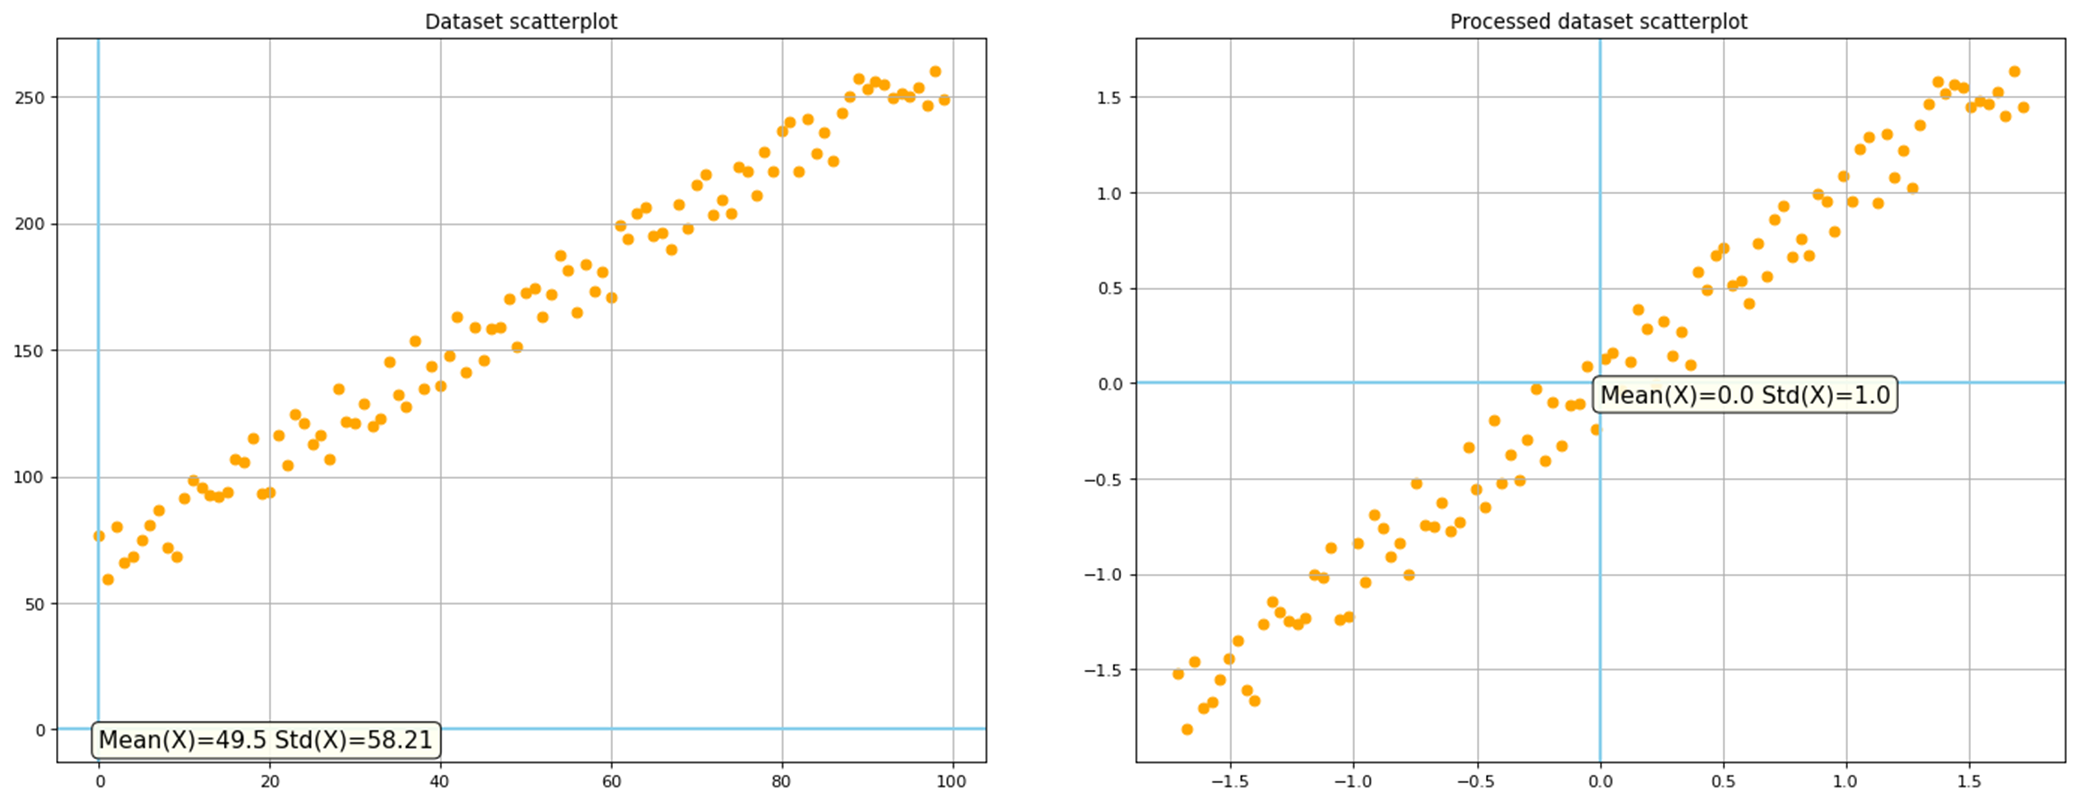
\includegraphics[width=0.9\textwidth]{SectionLetsMath/linearRegression_figures/fig_scalingCentering.png}
\captionsetup{type=figure}
\caption{Comparison between the original dataset and the centered and scaled one.}
\label{fig_scalingCentering}
\end{figure}

By switching the equation (\ref{eq_ridgeRegression}) to matrix form we have:

\begin{equation}
RSS\left(\lambda\right)=\left(y-X\beta\right)^T\left(y-X\beta\right)+\lambda\beta^T\beta
\label{eq_ridgeRegression1}
\end{equation}

The values of the ridge coefficients are calculated as follows.

\begin{equation}
{\hat{\beta}}_{ridge}=\left(X^TX+\lambda I\right)^{-1}X^Ty
\label{eq_ridgeRegression2}
\end{equation}

Compared to the  $\hat{\beta}$ coefficients of the linear regression, the ridge coefficients add $\lambda$ to the diagonal of $X^TX$. $I$ is a $P\times P$ identity matrix. Using the singular value decomposition (see section \ref{secSVD}) it is possible to express the least squared fitted vector and the solution of the ridge regression. In practice, $U$ spans the columns space of $X$, while $V$ spans the rows space of $X$ and $D$ is a diagonal matrix.

\begin{equation}
X{\hat{\beta}}^{ls}=UU^Ty
\label{eq_ridgeRegression3}
\end{equation}

\begin{equation}
X{\hat{\beta}}^{ridge}=UD\left(D^2+\lambda I\right)^{-1}DU^Ty
\label{eq_ridgeRegression4}
\end{equation}

In practice, it can be proved that the matrix $X^TX$ (which is similar to the sample covariance matrix $S=\frac{1}{N}X^TX$)  has been written using singular value decomposition matrix.

\begin{equation}
X^TX=VD^2V^T
\label{eq_ridgeRegression5}
\end{equation}

As already introduced in section \ref{secSVD}, the eigenvector $V$ describes the directions of the principal components of $X$. In practice, ridge regression shrinks the most the predictors having a small variance protecting against a potentially high variance estimated in the short directions (coefficients close to zero). The value of $\widehat{\beta\ }$ and the goodness of fit $r^2$ changes with different values of $\lambda$. Cross-validation can be used to identify the best value for $\lambda$.

\subsection{Lasso regression (L1-regularisation)} \label{secLassoRegression}
Lasso regression works similarly to Ridge regression, but it considers the minimisation of a different penalty function.

\begin{equation}
{\hat{\beta}}_{lasso}=\ argmin_\beta{\left\{\frac{1}{2}\sum_{i=1}^{N}\left(y_i-\beta_0-\sum_{j=1}^{N}{x_{ij}\beta_j}\right)^2+\lambda\sum_{j=1}^{p}{|\beta_j|}\ \right\}}
\label{eq_lasso1}
\end{equation}

Differently from ridge regression, the value of ${\hat{\beta}}_{ridge}$ cannot be computed directly since its computation is non-linear. Anyway, it can be efficiently computed through efficient algorithms to get a solution in a short time.\par

The lambda of a lasso regression can be determined using CV similarly to the lambda of ridge regression. Lasso regression penalty contains the $\hat{\beta}$ as well as ridge regression, but they shrink parameters differently.\par

Lasso regression can shrink a coefficient slope to 0. Increasing lambda, the bad-prediction parameters can go to zero (and the linked features are excluded from the model). Figure \ref{fig_regularisation} shows the effect of L1 and L2 regularisation on a 3-dimensional dataset.

% INSERT fig_regularisation
\begin{figure}[hbt!]
\centering
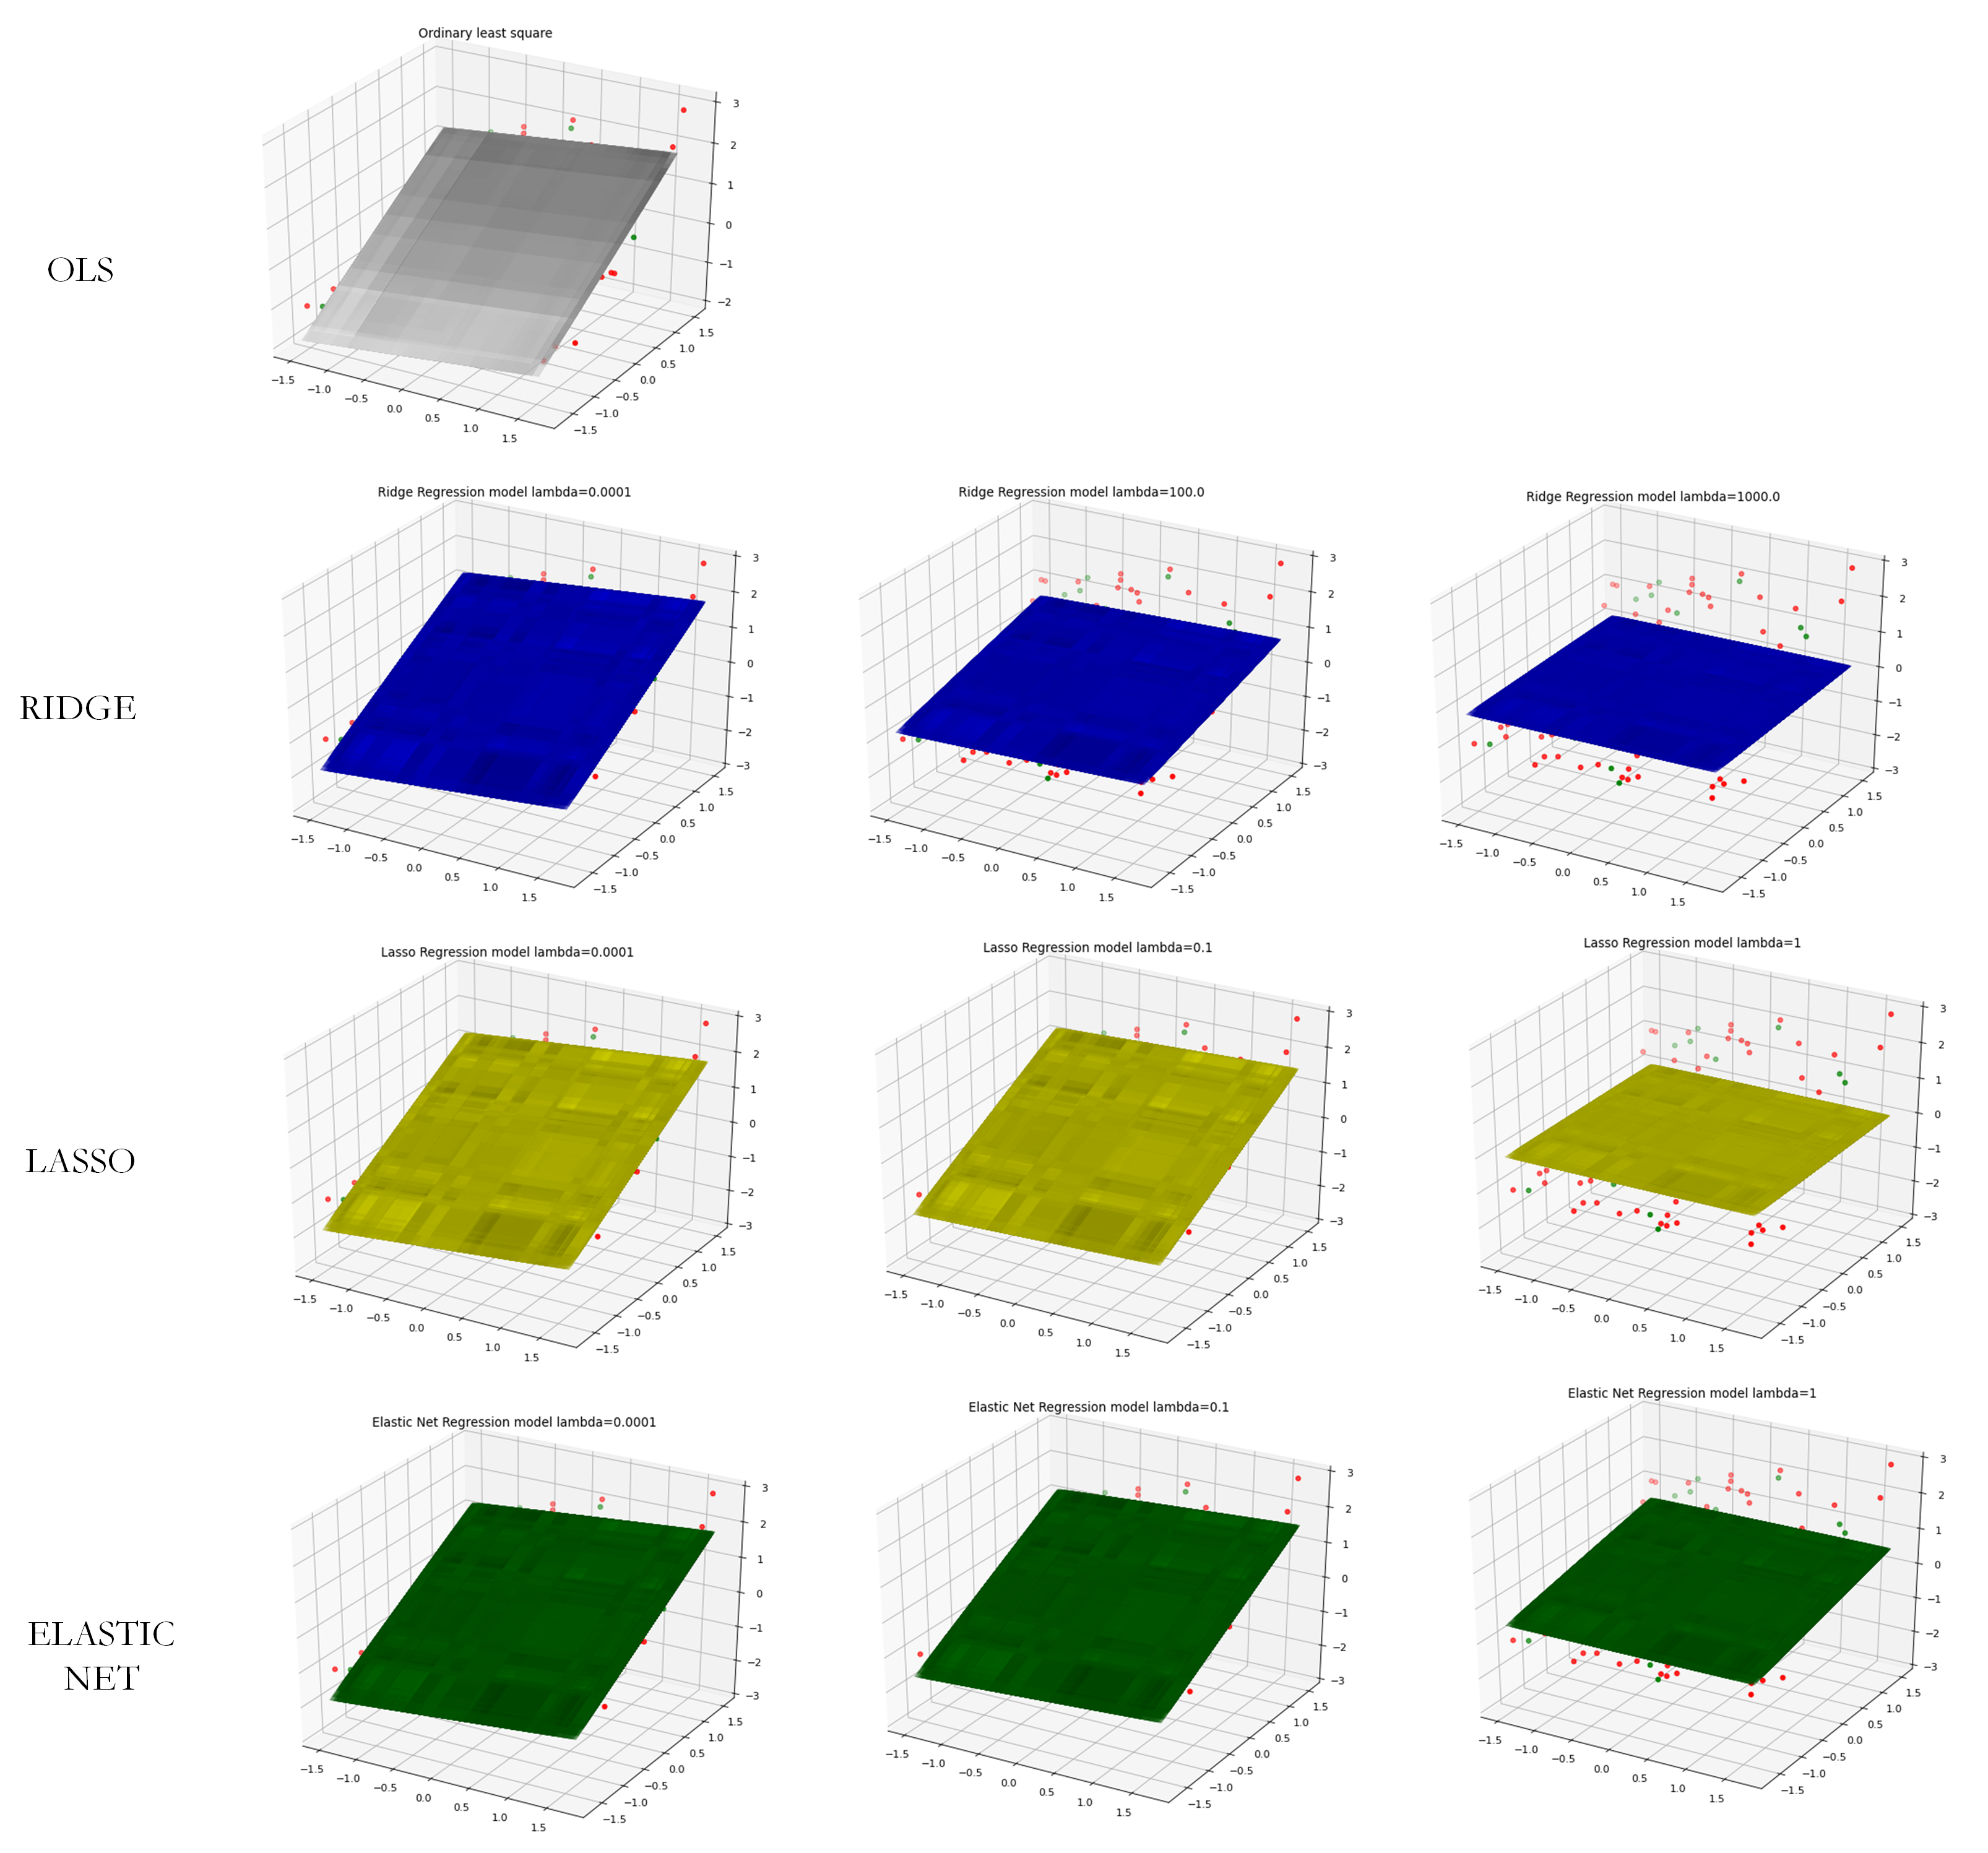
\includegraphics[width=0.9\textwidth]{SectionLetsMath/linearRegression_figures/fig_regularisation.png}
\captionsetup{type=figure}
\caption{Effects of the regularisation algorithms on the linear regression.}
\label{fig_regularisation}
\end{figure}


\subsection{Elastic-net regression}
When the number of parameters increases dramatically, elastic-net regression results adequate since it mixes the power of the Ridge and the Lasso. It is useful when a correlation between features exist since lasso can discard useless features, and ridge shrinks the correlated features together.\par

With elastic net regression, the parameters associated with the correlated variables are shrunk or removed all at once. The elastic-net penalty has the formula

\begin{equation}
\lambda\sum_{j=1}^{p}\left(\alpha\beta_j^2+\left(1-\alpha\right)\left|\beta_j\right|\right)
\label{eq_elasticnet}
\end{equation}

\subsection{Least angle regression}
This shrinkage method works as a forward stepwise regression (see section \ref{secForwardStepwise}) but it only enters “as much” of a predictor as it deserves. Its algorithm starts from a standardisation of the predictor. At each stage of the algorithm, it finds the predictor most correlated with the residuals, and it moves its ${\hat{\beta}}_j$ from 0 to its least-square coefficient until some other predictor has as much correlation as $j$. It continues until all the $j$ predictors have entered. 

\section{Derived input methods}
When the input is highly correlated, it could result convenient to preprocess the input first and then to apply a linear regression model

\subsubsection{Principal component regression}
This method applies the PCA first, to define a subset of $M<p$ orthogonal predictors, and then it performs the linear regression. It is important to standardise the input before applying PCA since it depends on its scaling. This procedure is similar to the Ridge regression, but it works discretely (it provides entire predictors) while ridge regression shrinks each coefficient.

\subsubsection{Partial Least Squares}
Partial Least square works similarly to the principal component regression. Nevertheless, while the principal component regression is based on the PCA and it gives higher importance to the directions having a higher variance, the partial least square seeks for the directions having both high variance and high correlation with the response.

\subsubsection{Transformation for linearity}
The assumption of a linear model (i.e., the function $f$ is linear in $y=f(X)$) often produces approximations on real predictions. It is always possible to transform the input data $X$ using a function $h$ before applying a linear model. In particular, the prediction model will be in the form:

\begin{equation}
y=f\left(X\right)=\sum_{m=1}^{M}{\beta_mh_m(X)}
\label{eq_transformationForLinearity}
\end{equation}
Common functions for $h_m$ are:
\begin{itemize}
    \item $h_m(X)=X_m$, no transformation on the initial data;
    \item $h_m\left(X\right)=X_j^2\ or\ X_jX_k$;
    \item $h_m\left(X\right)=\log{\left(X_j\right)}or\ \sqrt{X_j}\ $;
    \item $h_m\left(X\right)=I(L_m\le X_m<U_m)$, this case applies spline function to get a local polynomial approximation of the initial data.
\end{itemize}

Finding a function $h$ that linearise the relationship between $X$ and $y$ extends the field of application of the linear models.

\section*{Further reading}
Supplementary reading materials can be found in \cite{Skiena2017}, \cite{Igual2017}.

%\clearpage
\bibliographystyle{ieeetr}
\bibliography{SectionLetsMath/linearRegression_ref}